\chapter{Preliminary Evaluation of RTOS for RISC-V Based Hardware Accelerators}
\label{chapter:PreliminaryWork}
\section{Introduction}
% introdução ao trabalho que vou fazer
The purpose of this thesis is to study and evaluate the impact the use of a hardware accelerator has on an RTOS running on an SoC with a RISC-V based processor. This Chapter presents two initial solutions on how to manage a hardware accelerator with an RTOS. After that, it describes the experiments done to better understand the mechanisms of an RTOS. The first experiment was the development of a basic program that utilizes FreeRTOS capability to multitask. The developed program was then flashed into the board Raspberry Pi Pico. The second experiment was building the SoC SweRVolf using the Vivado Block Design Tool \cite{Vivado}. The last experiment was to run Zephyr in a simulation of the synthesized SoC.

The initial work done will help better understand how to design and build an SoC, making it easier for any future modification to the SoC. The installation of the two RTOS will help study the necessary procedures to incorporate a hardware accelerator into the RTOS. Finally, the use of already established hardware, such as the Raspberry Pi Pico board, helps to focus on the study of the RTOS mechanisms, without worrying about the correct use of the hardware.



\section{Integrating a Hardware Accelerator in a RTOS}
% Como é que o rtos vai ajudar com o acelarador?
% falar de alguns métodos que posso usar para incorporar o acelarador no rtos (reunião 2023/05/05)
Typically, when using hardware accelerators to improve processing performance, the CPU has to wait for the accelerator to finish it's job before continuing with it's execution. This results in a waste of processing time in the CPU since it will stay waiting for the accelerator to finish its work. One way to improve this is to implement a system that uses the CPU's resources while the accelerator is performing its work. The use of a RTOS should make this management much easier.

A first naive solution to be explored is to make use of the accelerator as if it was a function to be executed by the tasks. The communication between the task and the accelerator is managed by the task itself. This would mean a direct communication path, however, the task itself would have to make sure that the accelerator is not in use. If the hardware accelerator is already in use, the task would need a way to know when it is free. When the task manages to start using the accelerator it can free the CPU and allow other tasks to execute. In this solution, the accelerator will have to wake the sleeping task by triggering an event or interrupt. This interrupt is then perceived by the ISR that, in turn, will change the state of the task that needs the data from the hardware accelerator. This also means that the system will need to keep track of which task is waiting for the accelerator. Figure \ref{fig:sol1} shows a block diagram with the interaction of one task with the accelerator.

\begin{figure}[H]
    \centering
    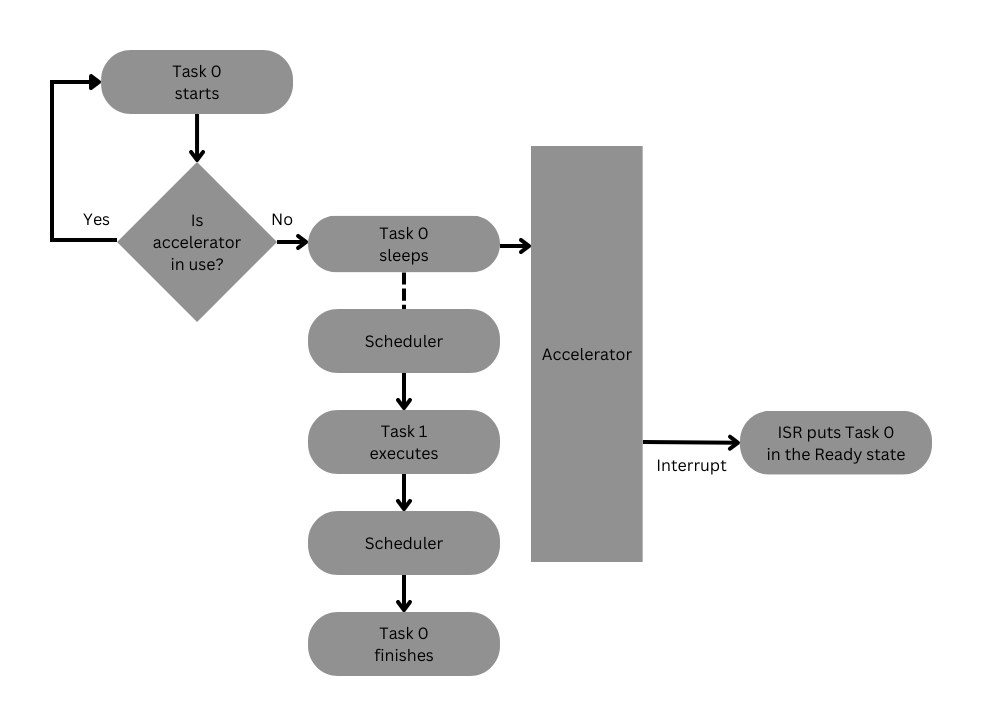
\includegraphics[scale=0.55]{Figures/sol1.png}
    \caption{Block diagram of a first naive implementation}
    \label{fig:sol1}
\end{figure}

Another solution is to have a specific task that manages the hardware accelerator. This would mean that anytime a task needs to use the accelerator, it must communicate with the task that controls it. The controller task can keep track of all the tasks that need the accelerator and manage its use. This will help reduce what the tasks need to do when they have to use the accelerator. However, this also adds overhead to the communication between the running task and the accelerator. The overhead exists because the task now needs to communicate with the controller task in addition to the communication between the controller task and the accelerator. Eventually, when the accelerator finished its work, the controller task can send the output to the original task. Figure \ref{fig:sol2} shows a block diagram with the interaction of one task with the task that manages the accelerator.

\begin{figure}[H]
    \centering
    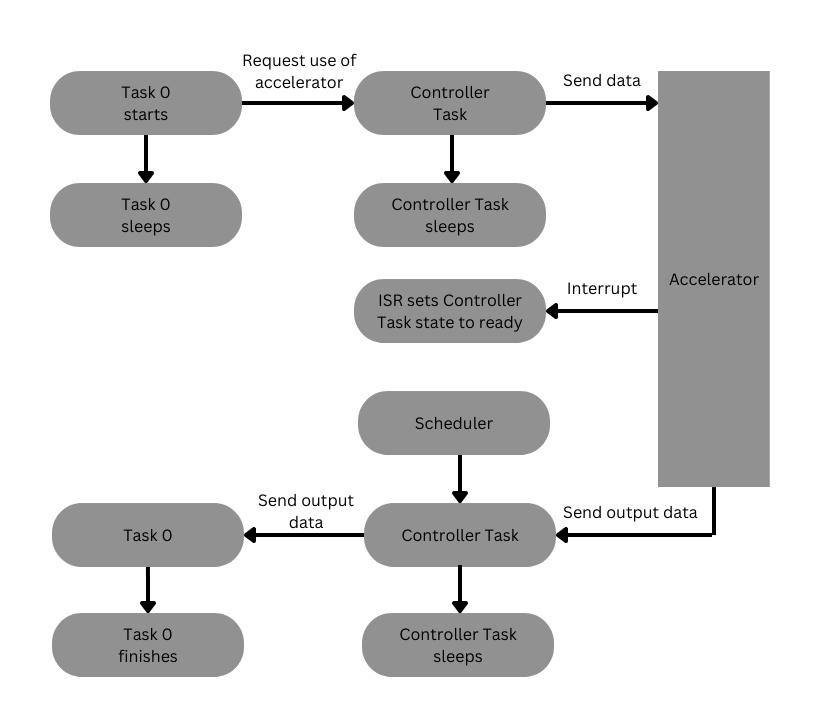
\includegraphics[scale=0.55]{Figures/sol2.png}
    \caption{Block diagram of a second naive implementation}
    \label{fig:sol2}
\end{figure}

\section{Preliminary Work}
% O que já fiz?
% Como é que o que já fiz ajuda o trabalho final?
The programs used and developed in this section can be found in the github repository \cite{gitrepo}.


\subsection{FreeRTOS on Raspberry Pi Pico}
The main objective of flashing a FreeRTOS program on the Raspberry Pi Pico is to understand the basic procedures necessary to implement custom programs. Since the Pi Pico is a commercial hardware platform, the documentation and support for the board are vast. The vast documentation also allows for a better understanding of RTOS mechanisms and how to use them, without needing to worry about configuring the RISC-V on the FPGA..

Before running any example programs, it was necessary to install the toolchain for the Pi Pico board. The Pi Pico toolchain allows developers to use the VSCode IDE with CMake to build the developed programs and generate the binary files. CMake is a tool that allows programmers to easily create binary files. The developer uses the CMakeLists.txt file to tell CMake how the program is structured and what libraries are necessary. After building the binary files, it is possible to flash the device and execute the programs.

The first two example programs to run were Blinky and Hello World. The Blinky example is a basic example that flashes the board LED repeatedly. The Hello World example is a basic example that prints "Hello, World!" to the serial monitor repeatedly. These examples demonstrate important capabilities of embedded systems: how to use GPIO, and how to use the serial monitor. The use of GPIO is essential for connecting extra modules to a system. The use of a serial monitor is essential for debugging and communicating information from the system to the user.

Finally, to execute programs with FreeRTOS the following steps were taken. First, create a new project with the FreeRTOS source code in the project folder. Second, add the path to the necessary libraries to the CMakeLists.txt file. These libraries include the file that ports FreeRTOS to the board and the file with the memory allocation instructions. The last step is to create the source files of the programs. The created program was a combination of the two examples programs already described. This program uses different tasks to blink the LED and to print "Hello, World!" to the serial monitor. Both of the tasks use timers that trigger the ISR when it's time to return to that task. The ISR then tells the scheduler that the task is ready to execute. The scheduler switches the execution context to the ready task. The task does its job and sleeps for a predefined time, waiting to execute when the timer triggers a new interrupt. In Figure \ref{fig:pico}, it is possible to see the Pi Pico flashing the LED and, in the background, the serial monitor with "Hello, World" being printed repeatedly.

\begin{figure}[ht]
    \centering
    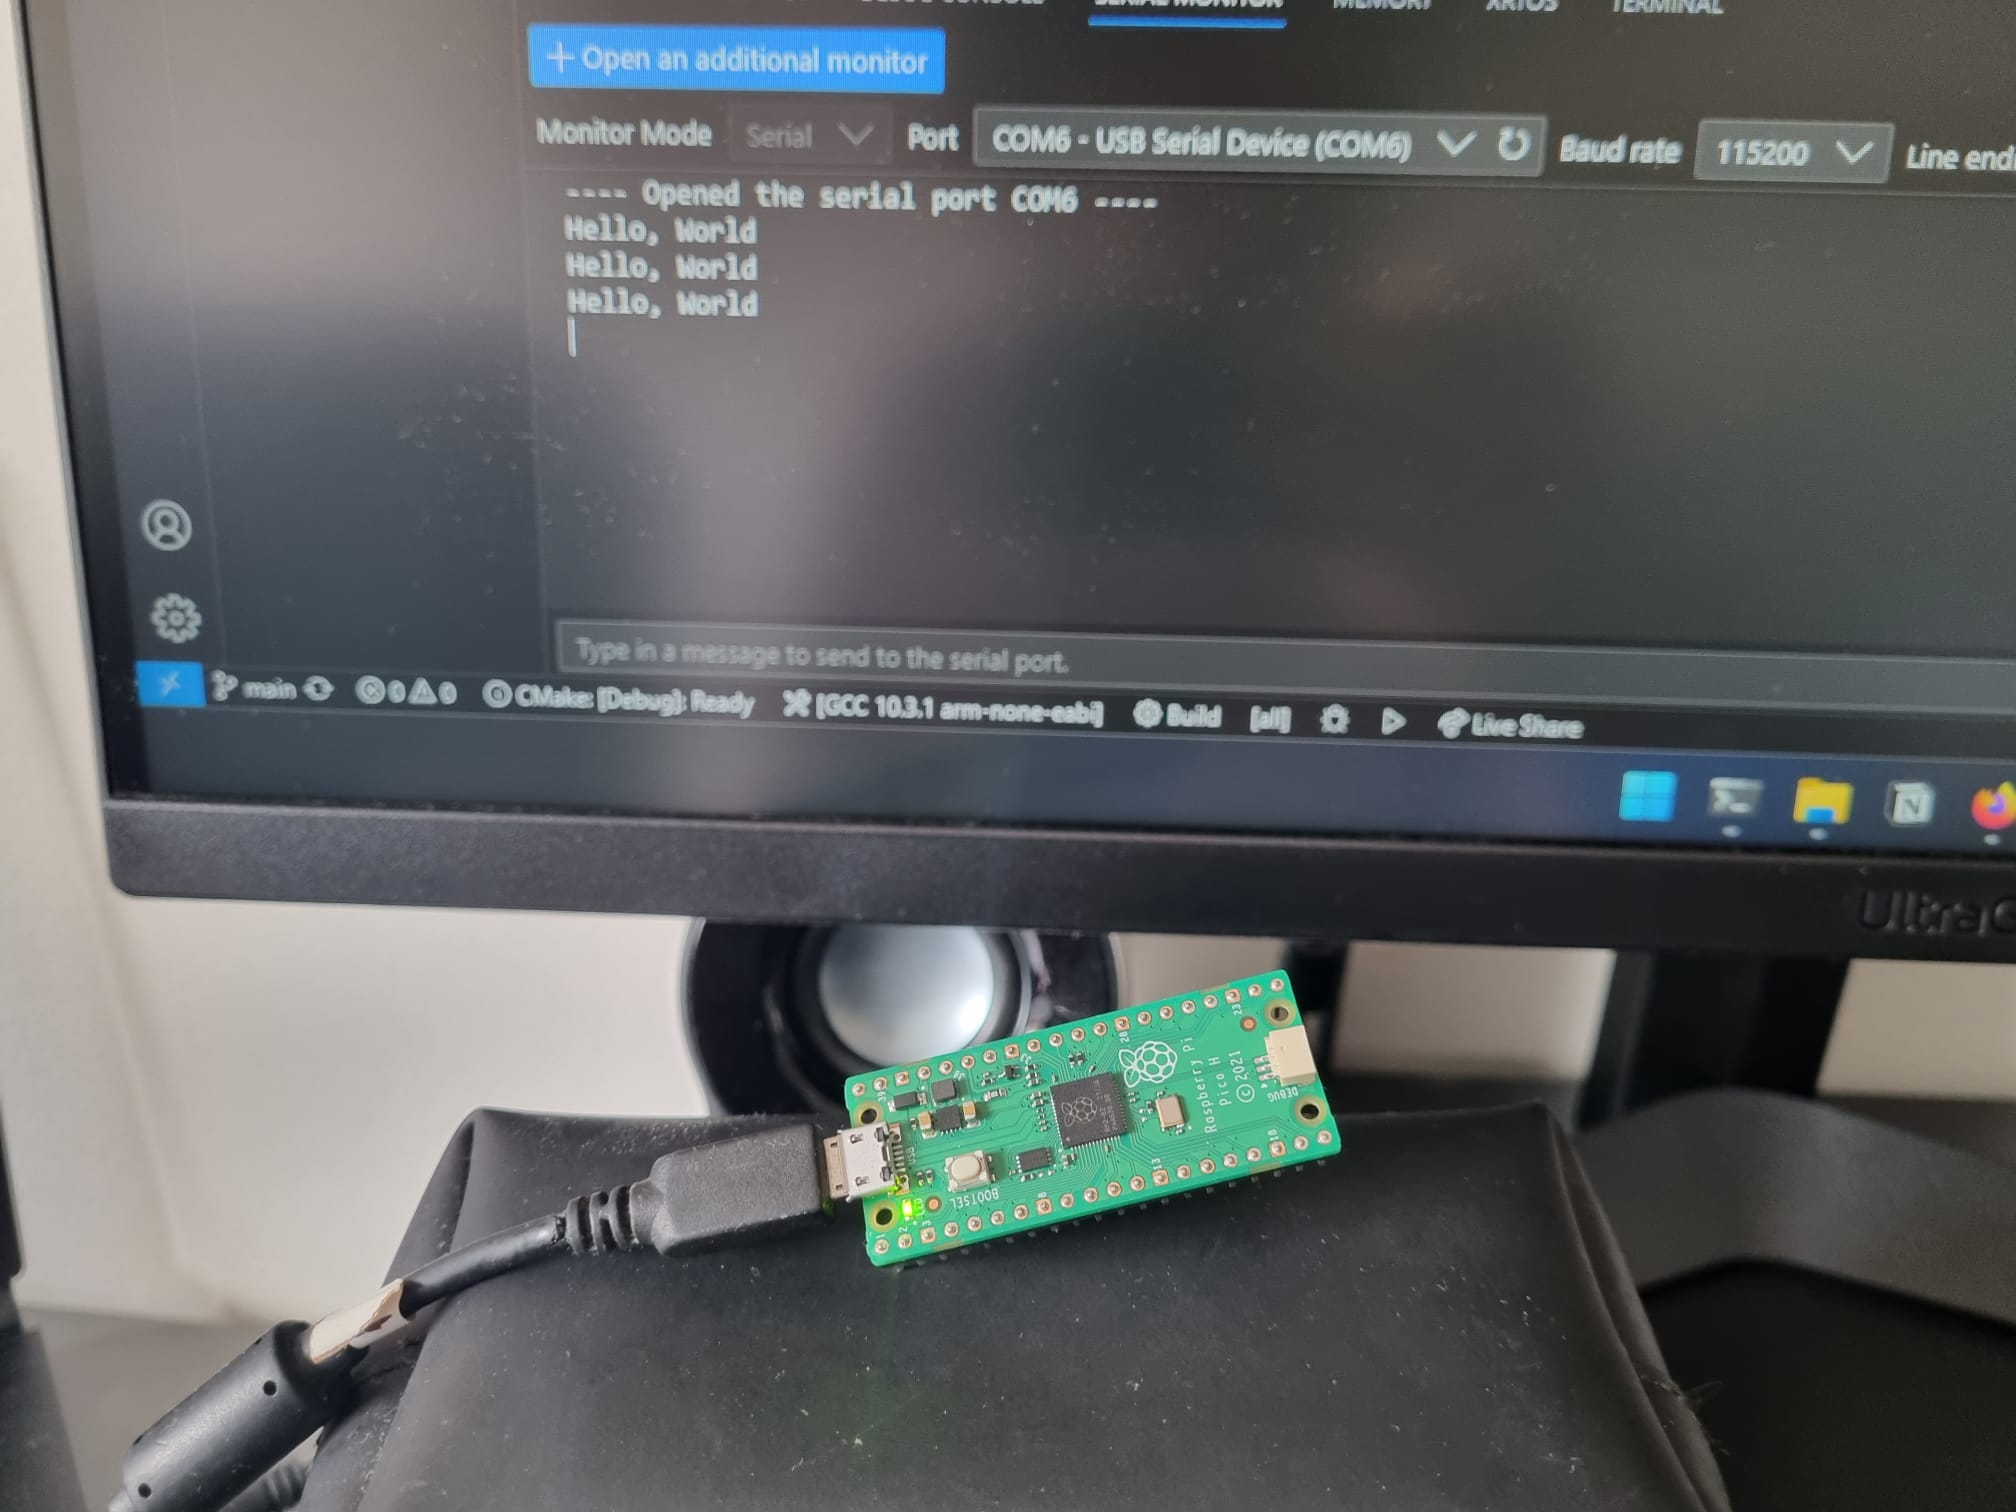
\includegraphics[scale=0.15]{Figures/pico-multitasking.jpeg}
    \caption{FreeRTOS executing on RaspberryPi Pico}
    \label{fig:pico}
\end{figure}

\subsection{SweRVolf SoC Synthesis}
To better understand how to build an SoC a subset of the SweRVolf was built using basic building blocks in the Vivado Block Design Tool. The SoC built is divided into three main major blocks: the SweRV Core, an Interconnect block (AXI Interconnect, AXI Wishbone Bridge, and Wishbone interconnect), and peripherals (System controller, Boot-ROM, and GPIO). Figure \ref{fig:SweRVolf} shows a block diagram of the SoC to be implemented.

\begin{figure}[ht]
    \centering
    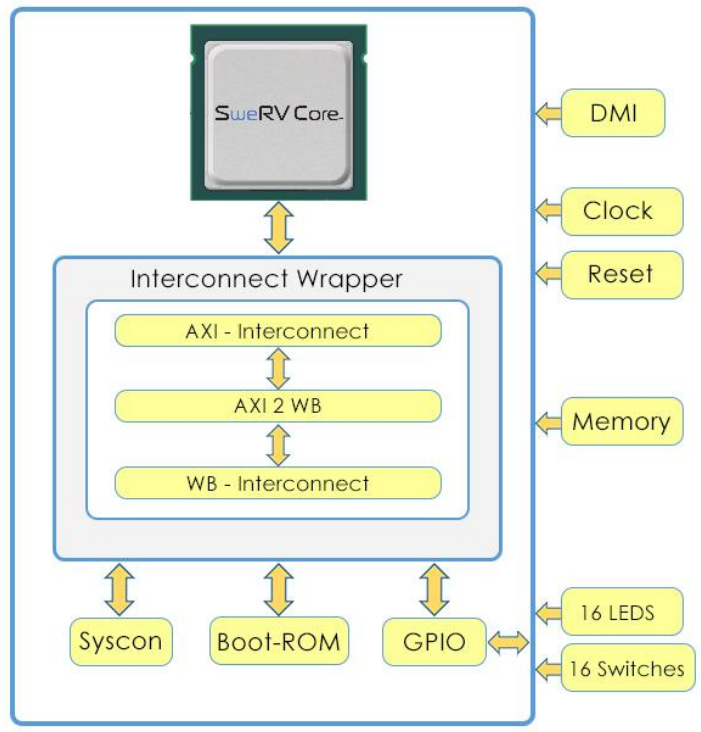
\includegraphics[scale=0.6]{Figures/SweRVolf.png}
    \caption{SweRVolf block diagram}
    \label{fig:SweRVolf}
\end{figure}

The first step to build the SoC is to create a project targeting the board Nexys A7-100T using Vivado. It's necessary to add all the individual modules to the sources of the project. These modules will map the connections so that the block design generated by Vivado can utilize the board components, for example, the LEDs and the switches. The second step is to create the block design and add the necessary modules: the SweRV Core wrapper module; the interconnect wrapper module, which contains the three interconnect modules; the Boot-ROM module; the GPIO module; the Syscon wrapper module that contains the system controller; and 32 bidirect modules, that will be attached to the GPIO and contain the 16 LEDs and 16 switches. The third step is to connect the different modules and add the external connections for the I/O pins. The external connections include the RAM, the clock, the reset, the debug module interface, and the bidirect GPIO modules. The last step is to synthesize the SoC and generate the bitstream file that will be used to configure the FPGA.


\subsection{Execution of Example Programs on the SweRVolf SoC}
Using PlatformIO \cite{platformio} and a binary file generated by Verilator \cite{Verilator} it is possible to build programs and simulate their execution on the SoC. Verilator uses the block design created in Vivado to generate the binary file for the simulation. It is now possible to create a PlatformIO project that will use the bitstream file created by Vivado and the binary file created by Verilator. The first PlatformIO project is a simple RISC-V assembly file that initializes the register t3 to 15 and subtracts 1 in every iteration of a loop until it reaches 0. Using the tool GTKWave it's possible to see the execution of the simple instructions. 

To run more complex programs with Zephyr it's necessary to install FuseSoC \cite{fusesoc}. FuseSoC is a package manager and a build system for HDL code. In this case, FuseSoC is the tool used to build the SweRVolf SoC and install Zephyr. With the full environment installed two example programs were executed. The "hello world" program is a standard program, used to ensure that the system is correctly built. After running the program with FuseSoC the expected output was printed to the terminal. 

The final program executed was the dining philosophers problem. The philosophers problem is an example problem that illustrates synchronization issues and how to solve them. This problem consists of five philosophers sitting at a round table with a fork in between each of them. The philosopher can be in one of three states: thinking, eating, or starving. To eat, a philosopher needs both forks on each side of him. The problem starts when two philosophers need the same fork to eat. This can create deadlocks. To solve this problem, the example program uses the Dijkstra's solution. The Dijkstra's solution introduces a "butler", which essentially provides a way to keep track of the available forks around the table. When a philosopher wants to eat, he requests the butler and when the forks are available the butler gives them to the philosopher. When the philosopher finishes eating, he signals the butler, who, in turn, assigns the forks to the next philosopher. This program correlates to the main problem of this thesis, which is how to best assign limited resources and when to put tasks to sleep while waiting for those resources.

% SE TIVER TEMPO DE FAZER: INSTALAR PROGRAMAS SIMPLES QUE USAM VÁRIAS THREADS E COMUNICAM ENTRE SI

\section{Conclusion}
% Quais vão ser as métricas de desempanho?
This Chapter introduces two solutions that will be explored in this thesis. In the first solution, the tasks communicate directly with the hardware accelerator. This solution has a smaller communication path between the task and the accelerator. However, this solution also increases the complexity of the tasks waiting for the accelerator. The second solution uses only one task to handle the communication with the accelerator. With a task controlling the communications, it is possible to use a queue to manage who needs to use the accelerator. The use of this task will add overhead between the communications, but reduce the complexity of each task requesting the use of the accelerator.

The second section of this Chapter reports the preliminary work done to better understand the inner mechanisms of an RTOS and the necessary procedures to build an SoC. The first experiment conducted was to use a commercial embedded system to execute an RTOS and develop skills in the use of tasks. The second experiment provided insight into how to design an SoC. This will facilitate the addition of different modules to the SoC. This Chapter also describes the steps taken for the use of simulators to execute Zephyr in the SweRVolf SoC. One of the programs executed was the philosophers problem. This problem illustrates how to manage a limited resource using the different mechanisms of an RTOS.


% RD: isto é o mais importante. é o que temos vindo a discutir
% introdução - explicar os ensaios/avaliaçoes
% 1 fase - explicar a escolha e utilização do rtos
% 2 fase - quais foram as configurações e porque
% 3 fase - como ficou e métricas de desempanho